\section{Introduction}
\label{introduction}

%Some do for fun, some do for money, some are insider attackers, and some are outsider adversaries.

Computer networks have become increasingly important components of people's everyday lives, and this trend seems poised to continue in the future. With this increased pervasiveness of networked systems
comes a commensurate increase in the number of people who attempt to break into them. Though a great deal of research effort has gone into preventing the exploitation of software vulnerabilities in order to
gain illicit remote access to computer systems, relatively little attention has been paid to interfering with attacks earlier in the attack life cycle, such as during the initial information gathering
stage. It has become increasingly difficult to monitor computer networks as they have grown in scale and complexity. This lack of awareness makes responding to, or even recognizing, attacks a challenge. As
a result, organizations' reactions to attacks are delayed, typically leaving them to address the situation long after an incident has taken place.

This work introduces the idea of creating a tool by utilizing existing network infrastructure features in order to provide Network Aware Defenses for Intrusion Recognition and Response (NADIR). The central
idea behind this research is to provide earlier notification of potential network attacks by using deceptive network service information  as bait. These ''decoy'' or ''honey-services'' will indicate system
weak points which do not exist when suspicious network circumstances are detected. That is, although up-to-date versions of the programs will be running on the system at all times, software versions with
vulnerabilities will be advertised when a potential attack or reconnaissance effort is detected. Attacks against these services will be unsuccessful because the server running our system is not actually
running the vulnerable services.

By providing fake vulnerable points, our system is capable of collecting information about attacks earlier in the reconnaissance phase, potentially catching adversaries in the act without exposing any
actual system weaknesses. Our solution effectively transforms any legitimate server into a ``honeypot'' without the added overhead of setting up and maintaining a set of fake network infrastructure.

In order to analyze network traffic to gain an understanding of contexts in which decoy service information should be deployed, we use a decision tree machine learning algorithm. Our system uses the Weka
machine learning toolkit \cite{misc:weka} to analyze, classify, and understand the structure of network traffic in order to infer when conditions are safe to reveal legitimate service details and when such
details should be masked with deceptive content.

%So that, we can move to the next step which is detecting and responding by using Snort \cite{roesch1999snort} in inline mode.

\begin{figure}[h!]
	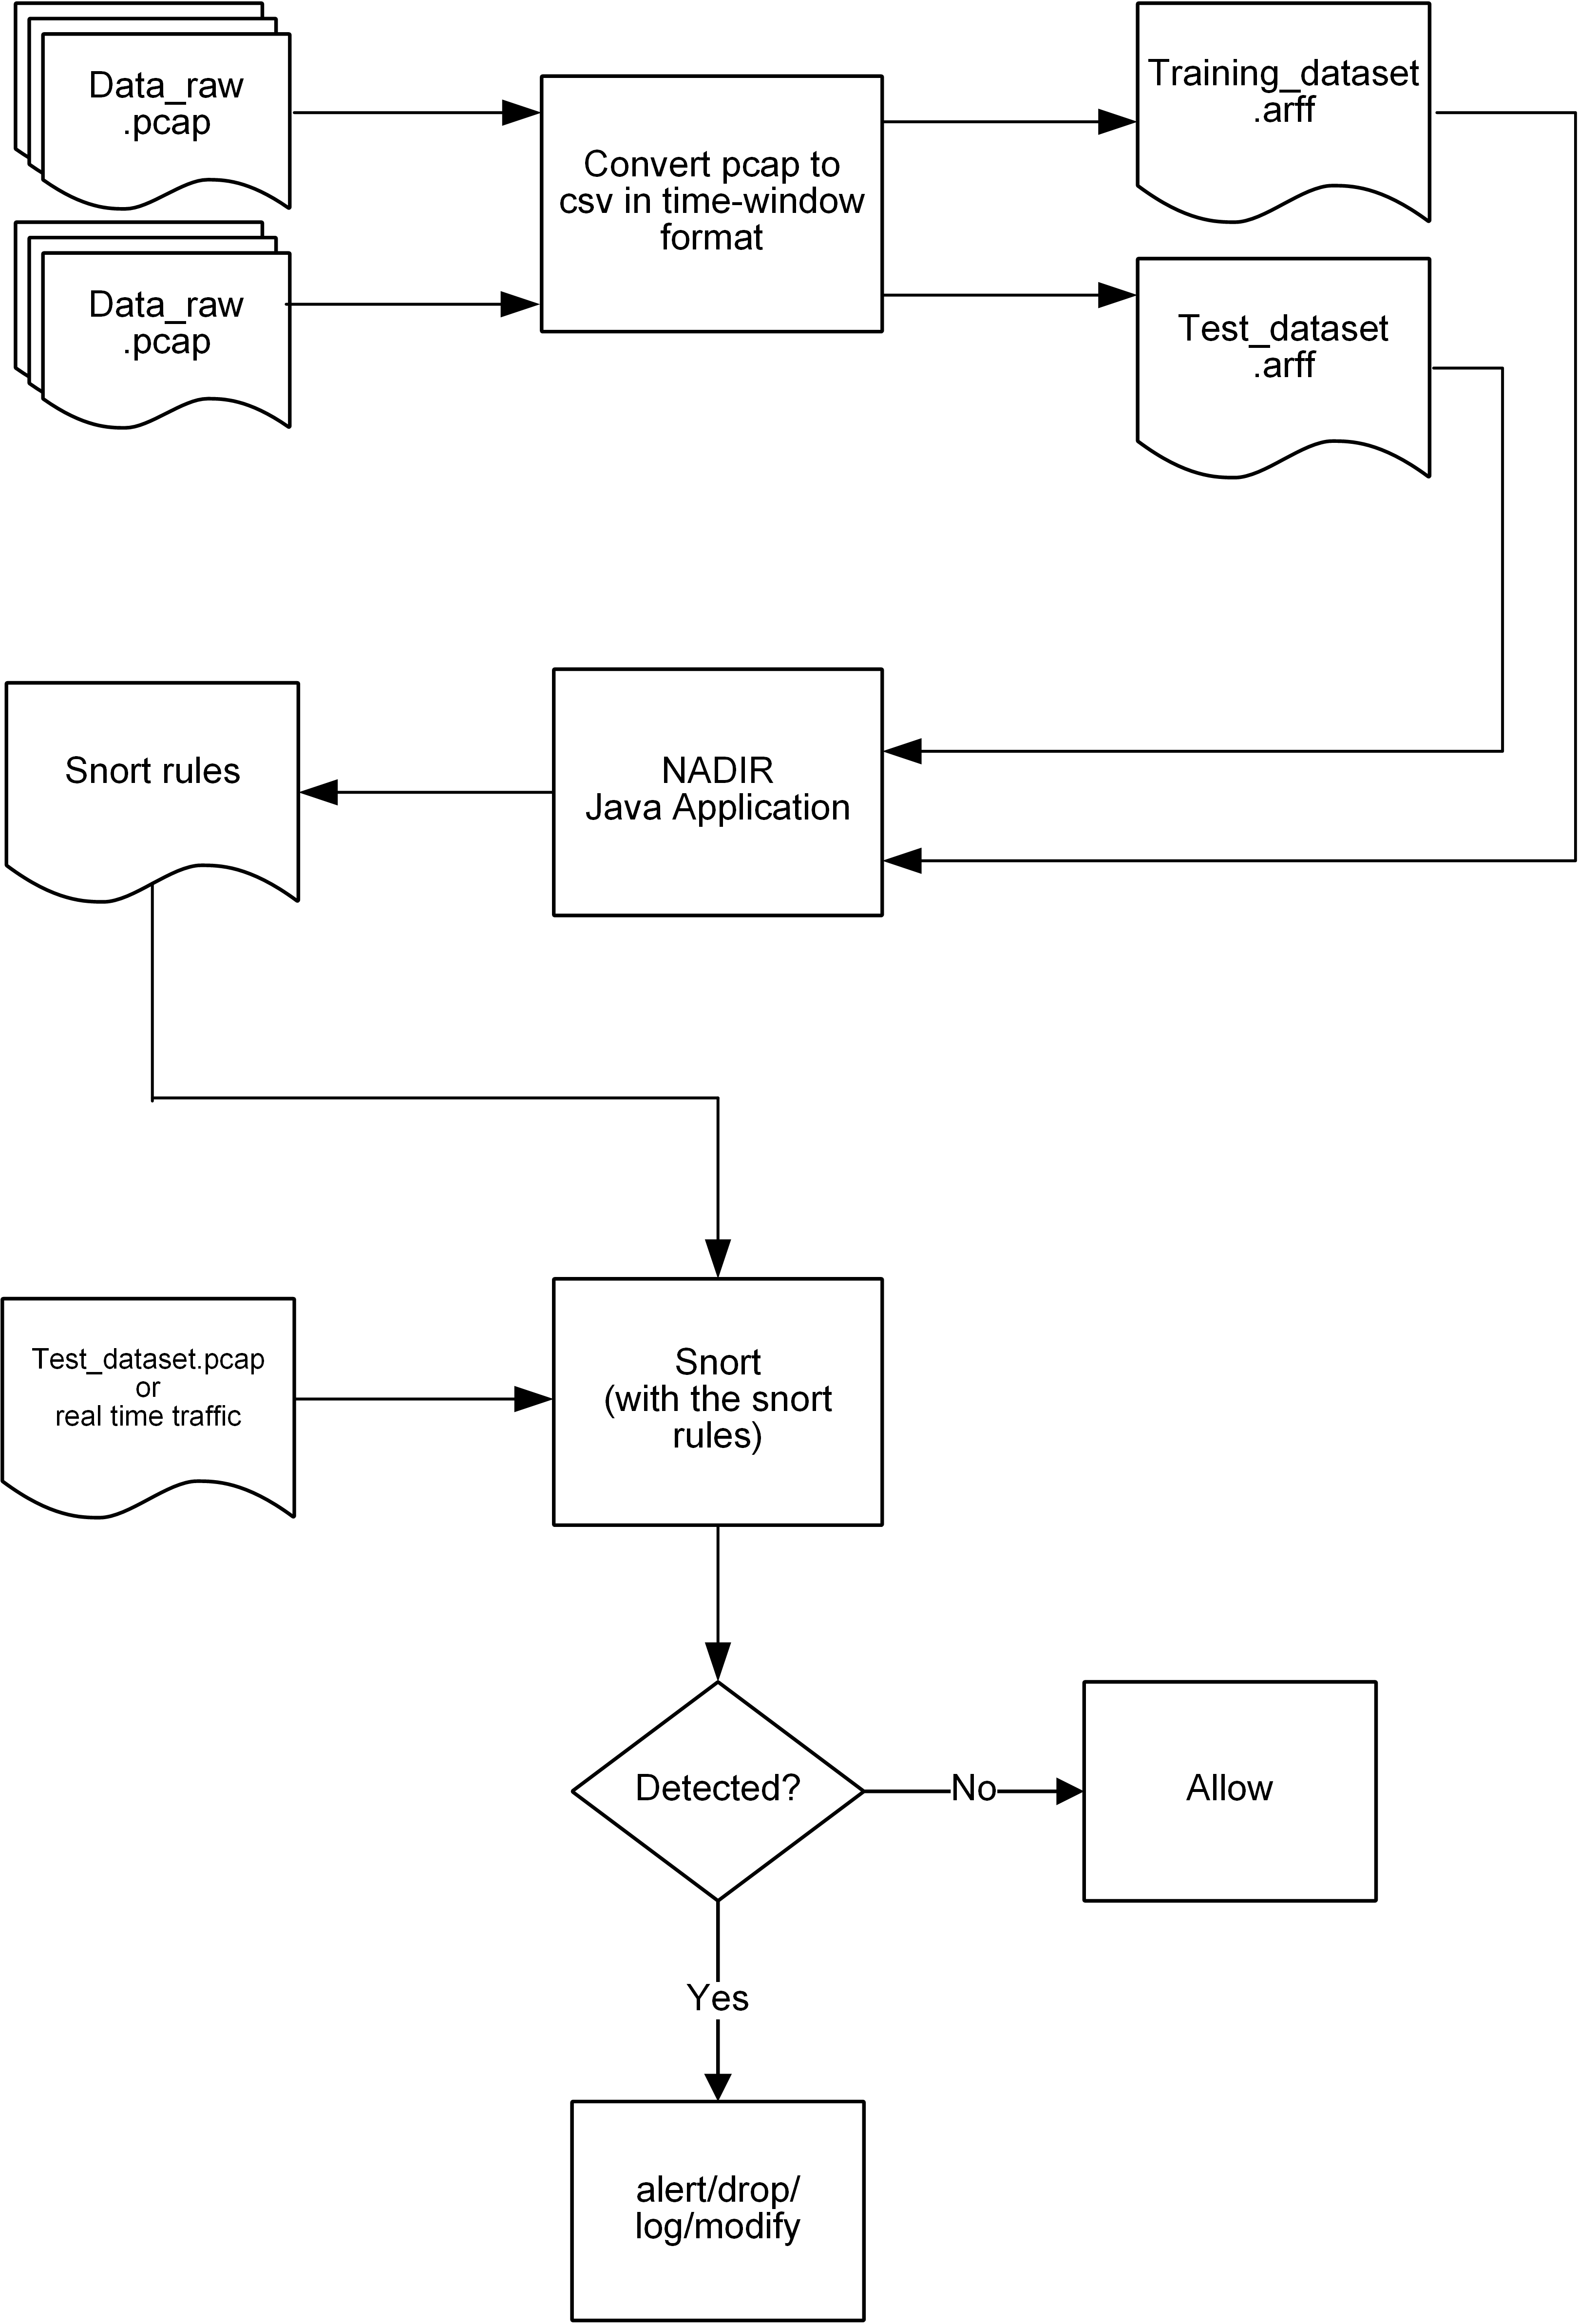
\includegraphics[width=\linewidth]{NADIR-processing_new_no_background.png}
	\caption{Over-all processing of NADIR System}
	\label{fig:overall}
\end{figure}

The overall workflow of our proposed system is shown as Figure \ref{fig:overall}. Our machine learning based technique is capable of classifying network traffic according to normal and abnormal patterns,
but several steps are required to process collected data prior to applying the classification algorithm. Firstly, we use an Intrusion Detection System (IDS) to collect network traffic data. In order to test
our system, we constructed a dataset comprised of the legitimate traffic observed by a test server on our university network as well as malicious traffic in the form of attacks we launched at known times to
provide ground truth.

Next, the collected network traffic data is converted into a Attribute-Relation File Format (ARFF) file for further processing. Subsequently, the NADIR system takes the network traffic data as input to
produces IDS rules based on what traffic was found to be indicative of an attack. Although any machine learning algorithm could potentially be used, we employed a decision tree classification algorithm to
produce IDS rules from the selected features automatically \cite{NetData2ARFF}. Finally, these rules are used to trigger our deception service description mitigation technique when unusual network
circumstances are detected.

The rest of the paper is organized as follows. Section \ref{related} discusses pertinent past research. Next, we present our threat model in Section \ref{threat_model}. The experiments we performed with our
system are presented in Section \ref{experiment} and their results are provided in \ref{results}. Finally, we conclude the paper in Section \ref{conclusion}.


